%\documentclass[11pt]{article}
\documentclass{report}
\usepackage[nottoc,notlot,notlof]{tocbibind}
\usepackage[english]{babel}
\usepackage{graphicx}
\usepackage{amsmath}
\numberwithin{figure}{section}
\usepackage{setspace}
\usepackage{subcaption}
\usepackage{enumerate}
\usepackage[export]{adjustbox}
\setstretch{1.5}
\usepackage{url}
\usepackage[title,titletoc,toc]{appendix}
\usepackage[font=small,labelfont=bf,justification=raggedright,singlelinecheck=false]{caption}
%%%%%%%%%% Start TeXmacs macros
\setlength{\voffset}{0.3in}
\setlength{\textheight}{8.5in}
\setlength{\topmargin}{-0.5in}
\setlength{\headheight}{0.0in}
\setlength{\headsep}{-0.0in}
\setlength{\footskip}{0.8in}
\flushbottom
\setlength{\textwidth}{5.6in}
\setlength{\oddsidemargin}{0.5in}
\setlength{\evensidemargin}{0.5in}
\setlength{\columnsep}{2pc}
\setlength{\parindent}{1em}
%%%%%%%%%% End TeXmacs macros

\usepackage{authblk}
\usepackage{hyperref}
\usepackage{refstyle}

\begin{document}
\title{CS 6630: Project Process Book
	\\TED talks topic trend visualization\\}
\author{Hsuan Lee}
\author{Chien-Wei Sun}
\affil{School of Computing, University of Utah}

\maketitle

\tableofcontents{}
\chapter{Overview}
\section{Overview and Motivation}

\quad TED is a leading organization which provides influential and understandable talk to the world. These talks cover a lot of fields, from anthropology to machine learning, and also from biology to sociology. We are interested in the relationship between technology and world market, and we want to know if TED somehow shows the trend of popular technology or it provides a platform for topics which do not get much attention in the world. 

\quad The relevance of different categories is also what we want to discover. For example, several years ago, it was popular that researchers tried to innovate theory according to the behavior of insects, like ants and bees. There are many theories developped based on the cooperation pattern of those animals. In the past, people did not consider that there is a strong relevence between insects and learning theory. We also wonder if we can find situation which is similar to the example.

\section{Related Work}

\quad When we are searching useful data for this project, we found the TED talks dataset and also a visulization by Sean Miller\cite{prework}. In this visualization, it shows statistics of the dataset and also allow user to search video by one tag. However, this visualization does not answer the questions we mention in the above. That's why we decide to build our own visualization of the dataset.


\section{Questions}
\quad Here are questions we expect to answer at the end of this project:
\begin{itemize}
\item
What are the trend of category tags appeared on TED talks?
\item
Is there any relationship between the TED talks and the big events happened in the world? 
\item
Is there a strong relevence between two topics that in general people will not think they are related?
\item
Can we learn the trend of research on a specific field by analyzing the popularity of keywords? Or it shows the topics which people do not put attention on for now but will become important in the future?
\end{itemize}

\chapter{Data}
\section{Dataset}

\quad We find the dataset from Dataset Distribution Portal\cite{idiap}.
This dataset include the video recording from the TED website from 1972 to 2017. For each video, its data contains the following attributes:{}
\begin{figure} [h]
\begin{center}
\includegraphics[scale=0.4]{"csv"}
\caption{Data get from idiap.ch}
\label{fig:csv}
\end{center}
\end{figure}

\begin{center}
\begin{tabular}{l|l}
id & month filmed \\
Speaker & year filmed\\
headline & event\\
URL & duration \\
description & date published \\
transcript URL  & tags \\ 
 \end{tabular}
\end{center}

%\clearpage

\quad To better understand the impact of TED videos, we develop web crawlers to collect attributes like \textbf{rates}(how do people feel after watching a video), \textbf{views}(how many time a video has been played), and some potentially valuable data like datetime, redirected urls, and transcripts. We use \textbf{Scrapy}\cite{scrapy}  as our crawler. Figure~\ref{fig:ratethistalk} displays the rating options on TED website.

\begin{figure} [h]
\begin{center}
\includegraphics[scale=0.4]{"ratethistalk"}
\caption{How people rate one video in TED website}
\label{fig:ratethistalk}
\end{center}
\end{figure}

Furthermore, in order to load data easily, we transfer our data from csv file to json form. We found this preprocessing can be accomplished painlessly by using  \textbf{Pandas}\cite{pandas} toolkit. Figure~\ref{fig:jsonofvideo} shows what kind of data one video contains.

\begin{figure} [h]
\begin{center}
\includegraphics[scale=0.4]{"onevideodata"}
\caption{Data of one video in JSON}
\label{fig:jsonofvideo}
\end{center}
\end{figure}

\quad We plan to visualize the data according to the tags/keywords of the video. It is not efficient to search all the data to find which videos are related with one specific tag on javascript. For practical implementation, we will preprocess the dataset based on tags, which means to use tag as key to create input data.

\section{Exploratory Data Analysis}

\quad In our design, the main chart user interact with is the network chart, which present the co-occurrence of tags. Hence, after we finish the job of collecting data, we move forward to build the co-occurrence matrix of tags. During this procedure, we observe that some tags appear in too many videos so that their existences are not meaningful to the matrix. These tags are `science', `technology', `global issue'. Since they show up in most of talks, we remove them from the matrix so that the network chart will look clear.

\quad To create groups of tags, we apply k-means to divide them into 11 clusters, and one of them restore the outliers. Figure~\ref{fig:group} are the results of two groups. One is the group whose center is tag `computers', the other is the group whose center is `universe'. Color is used to distinguish the group in our design.
\begin{figure} [h]
\begin{center}
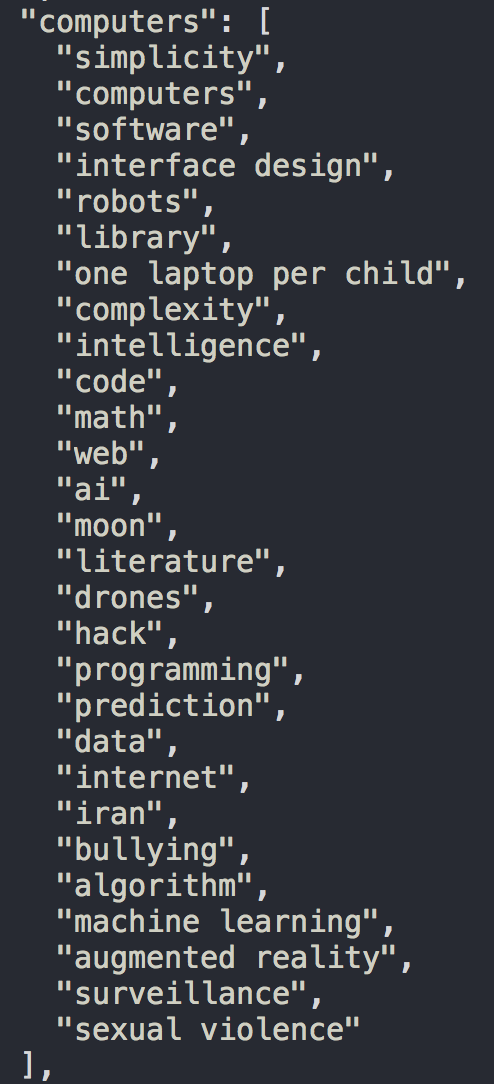
\includegraphics[scale=0.5]{computersgroup}
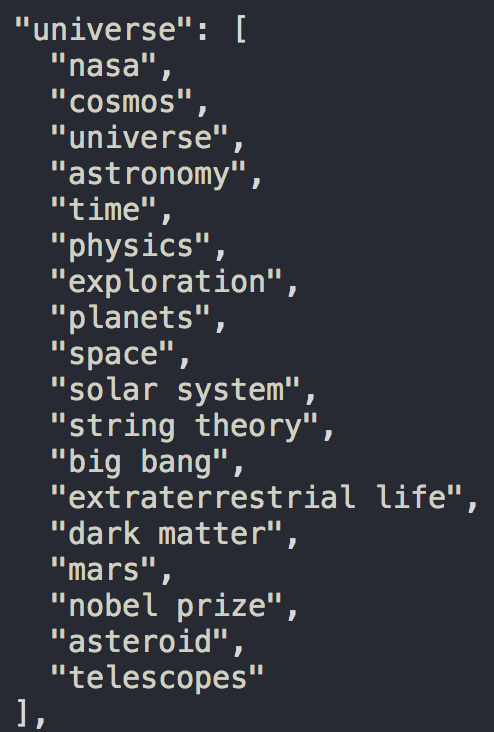
\includegraphics[scale=0.5]{universegroup}
\caption{Clustering result}
\label{fig:group}
\end{center}
\end{figure}
%\clearpage

\chapter{Design Evolution}

\section{Prototype}
\quad Our design is based on the network layout, as shown in Figure~\ref{fig:design1}. This network is composed of tags, and user can choose several tags they are interested in to through interaction with the network node. Next, the line chart in the middle of Figure~\ref{fig:design1} will display the tendency of chosen tags versus time/year. The last part help user to search for TED talks including these tags. User can decide the result is sorted by views or popularity.

\begin{figure}
\begin{center}
\includegraphics[scale=0.12]{"IMG_9010".JPG}
\caption{Design draft}
\label{fig:design1}
\end{center}
\end{figure}

\begin{figure}
\begin{center}
\includegraphics[scale=0.12]{"IMG_9011".JPG}
\caption{Design of Optional features}
\label{fig:design2}
\end{center}
\end{figure}

\quad We also want to compare the statistic of the tags between years, so we design a bar chart as shown in Figure~\ref{fig:design2}. By making use of the sliding bar on the top, the statistics of two years is displayed. Figure~\ref{fig:data} helps us to figure out what attributes are needed in each chart. It also shows the relationship of charts.  

\begin{figure}
\begin{center}
\includegraphics[scale=0.8]{"Untitled Diagram".png}
\caption{Category of data, and it relationship with the layout}
\label{fig:data}
\end{center}
\end{figure}

\section{Evolution}

\subsection{Network Chart}
\quad First, we generate the network chart accoring the co-occurence matrix. Each node represent a tag, and the thickness of one link is decided by the co-occurence value between two tags. However, there are 403 tags and 19488 links on this chart, which make the network look crazy and take a lot of time to draw these lines, as shown in Figure~\ref{fig:networkball}. 

\quad We discuss how to fix this issue and propose two solution for that. One is to draw chord layout in the beginning. Chord layout help people understand the relationship between two groups. We can let user to click ribbon to then show the network layout of tags in these two groups. However, this design does not allow us to observe all the related tags of one tag we choose. The other solution is to reduce the amount of links and nodes. We can provide an overview of network chart with nodes and links whose frequencies and value of co-occurence are bigger than threshold. Then, to zoom in on this chart, user can double-click on the tag they interested in to find all the other tag which is related to the chosen one. After applying the second method, our network chart looks better, as you can find in Figure~\ref{fig:networkwithcolor}.
\begin{figure}
\begin{center}
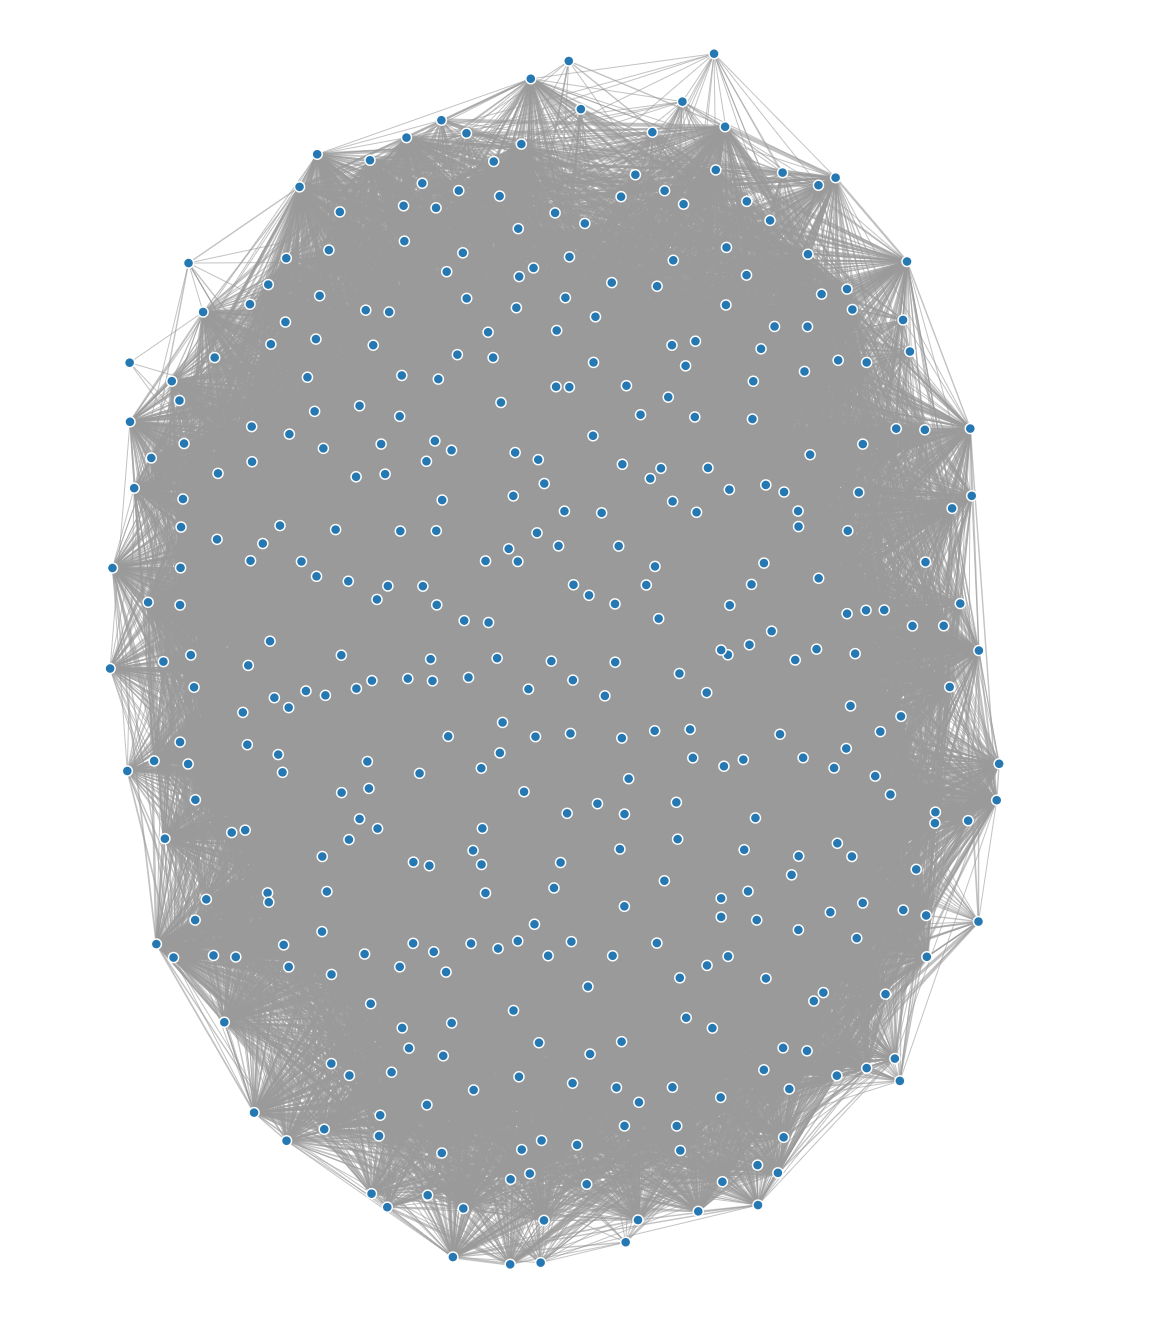
\includegraphics[scale=0.3]{Crazylink}
\caption{Network chart with Over 19,000 links}
\label{fig:networkball}
\end{center}
\end{figure}

\begin{figure}
\begin{center}
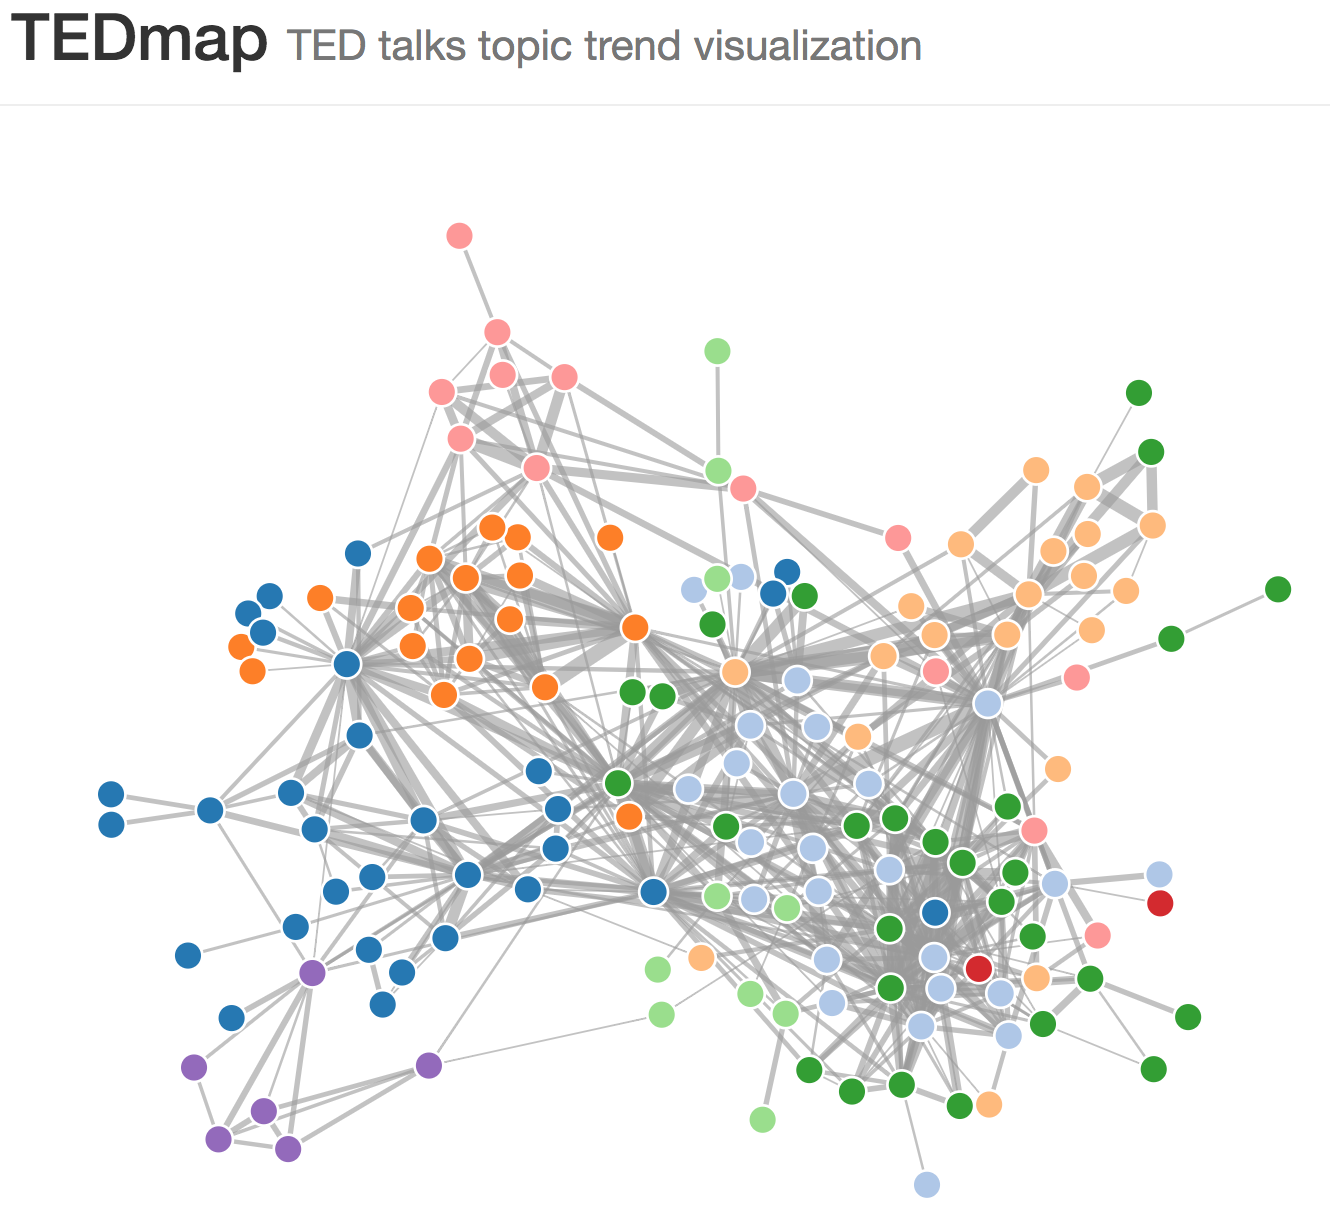
\includegraphics[scale=0.4]{networkChartProto}
\caption{Network chart with link vale bigger than 15}
\label{fig:networkwithcolor}
\end{center}
\end{figure}	

\quad Next, we want to observe the relationship between a chosen tag and other co-occurrence tags, so we implement a function that the network chart shows all the links whose edges include a specific tag after double-clicking on one the corresponding node. The image was not easy to understand and hard to find the most relative tag, as shown in Figure~\ref{fig:zoomin1}.

\quad Figure~\ref{fig:zoomin2} is the modified design to solve the above issue. This time, we grouped all the related tags by their categories. Instead of connecting the center with relative node, we connect it to an invisible group center and then link node with the center. This design help user to learn which category has strong co-occurrence within the specific, and also it is obvious to observe the most related tag. We call it \textbf{flower chart}, and this term is used to describe network chart within selected center in the following content.

\quad To show the tag name of each node, we decide to apply tooltip instead of adding text to them. Also, to avoid the situation that the tooltip goes beyond the border, the direction of d3-tip is set to southwest. The information we provided in tooltip depend on whether it is flower chart or not. If network chart is not shown as flower chart, we will paste the tag name and the top five strong related tags and co-occurrence with the node we hover on. Figure~\ref{fig:tt1} is an example when the mouse hover on node which present `biology'. If the chart becomes flower chart, then tooltip shows the tag name and co-occurence while we hover on that node, as you can see in Figure~\ref{fig:tt2}. Stroke width and color are changed to highlight which node we are watching.   

\quad Now this question comes to our mind: what if we want to know the co-occurrence between two tags in one year? To answer this this question, we add an button on the upper-right corner to let users choose which year they want to observe, as displayed in Figure~\ref{fig:yeardropdown}. Example in Figure~\ref{fig:compareyear} demonstrate the comparation between 2003 and 2012.

\begin{figure}
\begin{center}
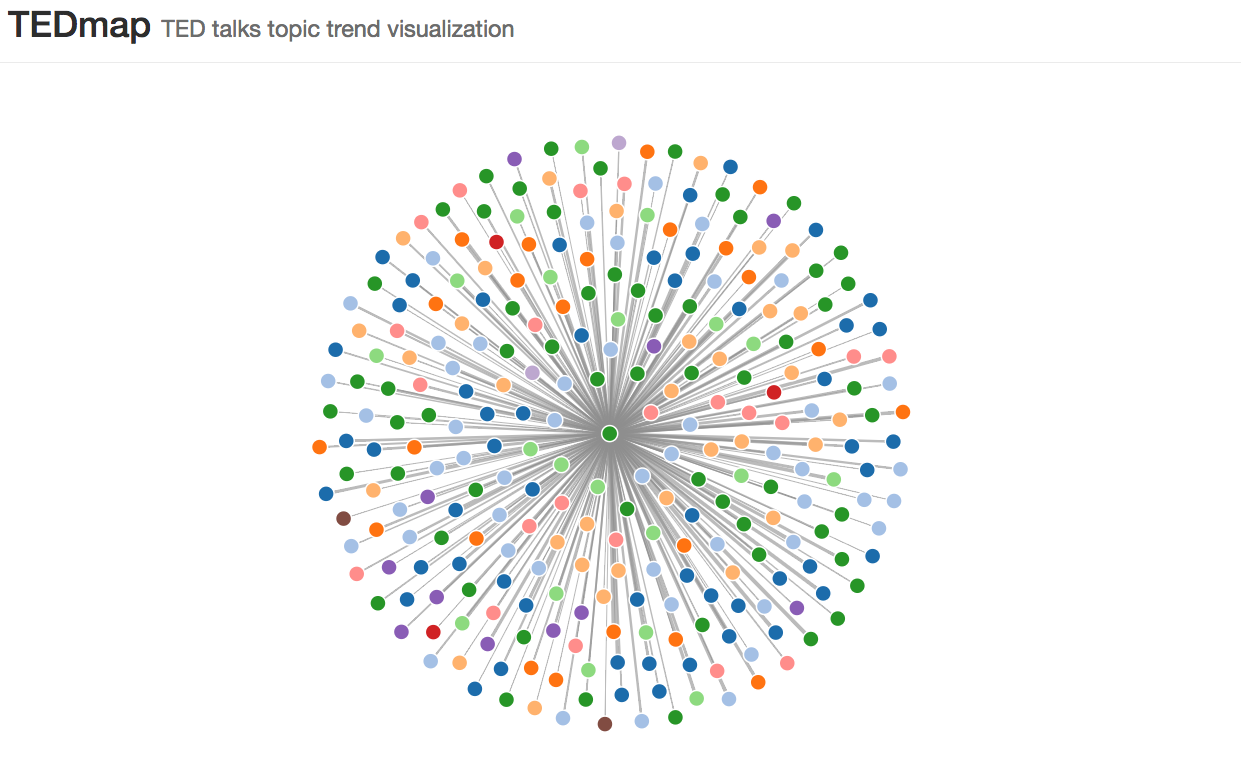
\includegraphics[scale=0.25]{focusOneTag_d1}
\caption{Zoom in for one tag}
\label{fig:zoomin1}
\end{center}
\end{figure}

\begin{figure}
\begin{center}
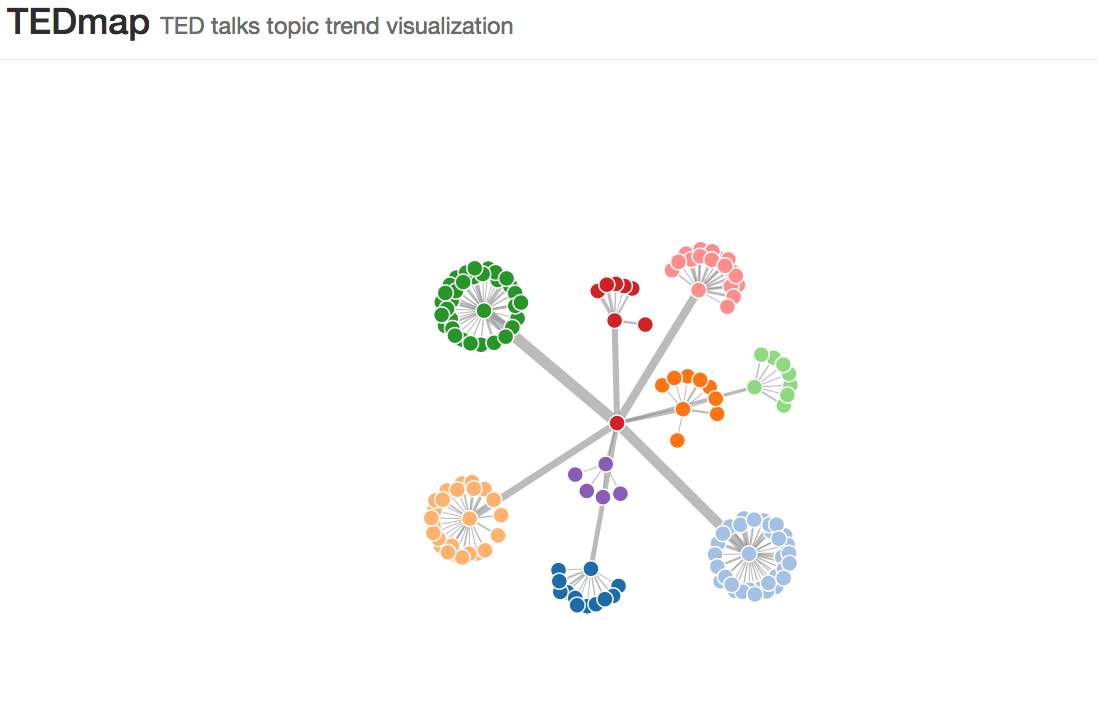
\includegraphics[scale=0.3]{focusOneTag_d2}
\caption{Zoom in for one tag with grouping}
\label{fig:zoomin2}
\end{center}
\end{figure}

\begin{figure}
\begin{center}
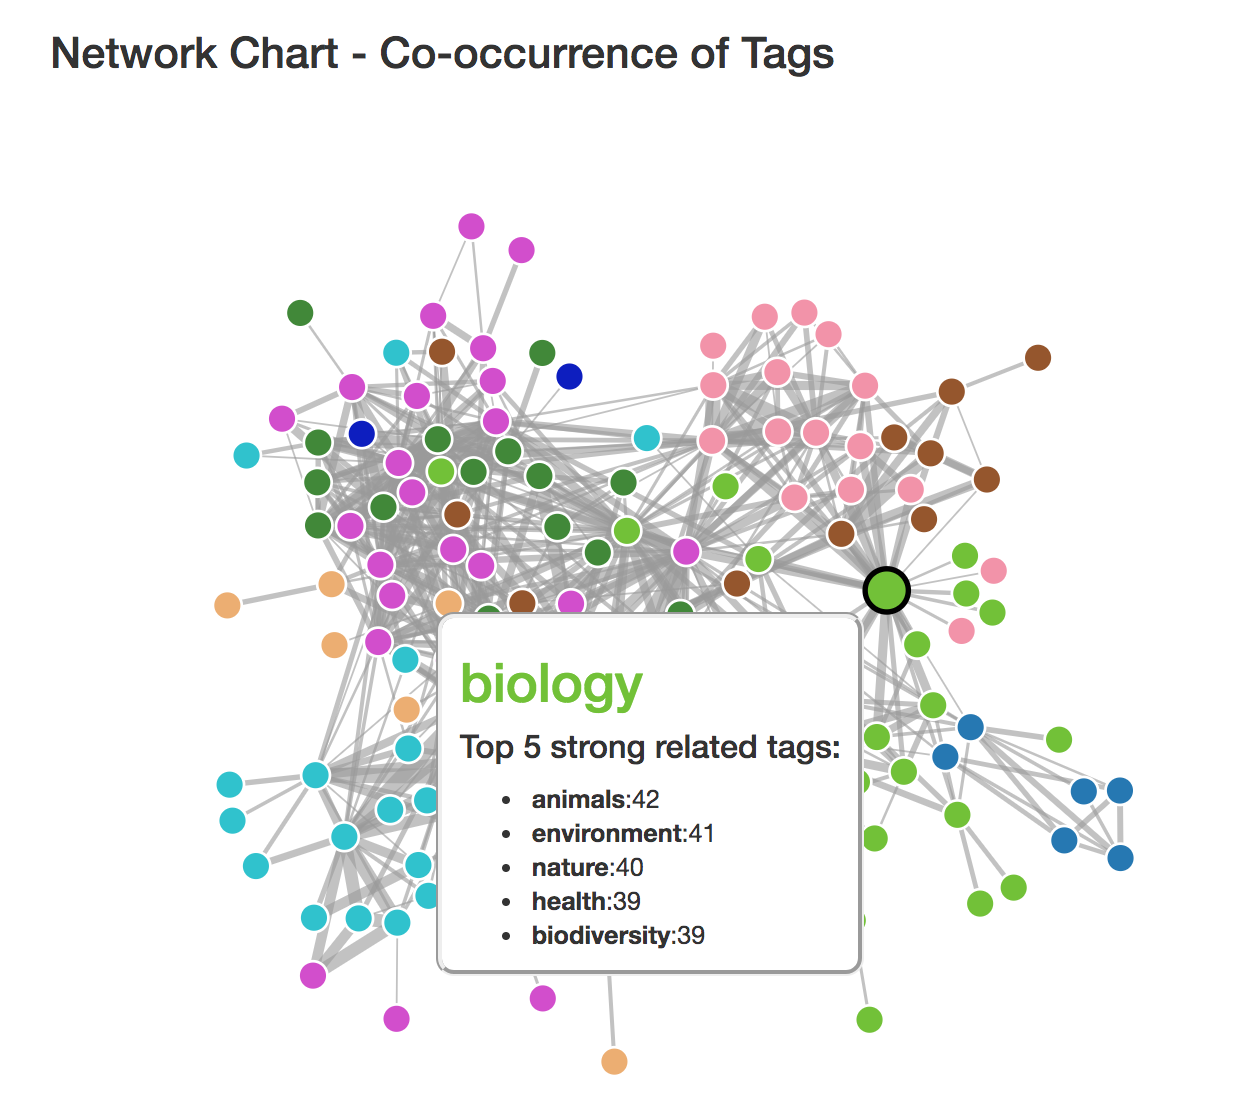
\includegraphics[scale=0.5]{top5tooltip}
\caption{Tooltip design when no tag are focused on}
\label{fig:tt1}
\end{center}
\end{figure}

\begin{figure}
\begin{center}
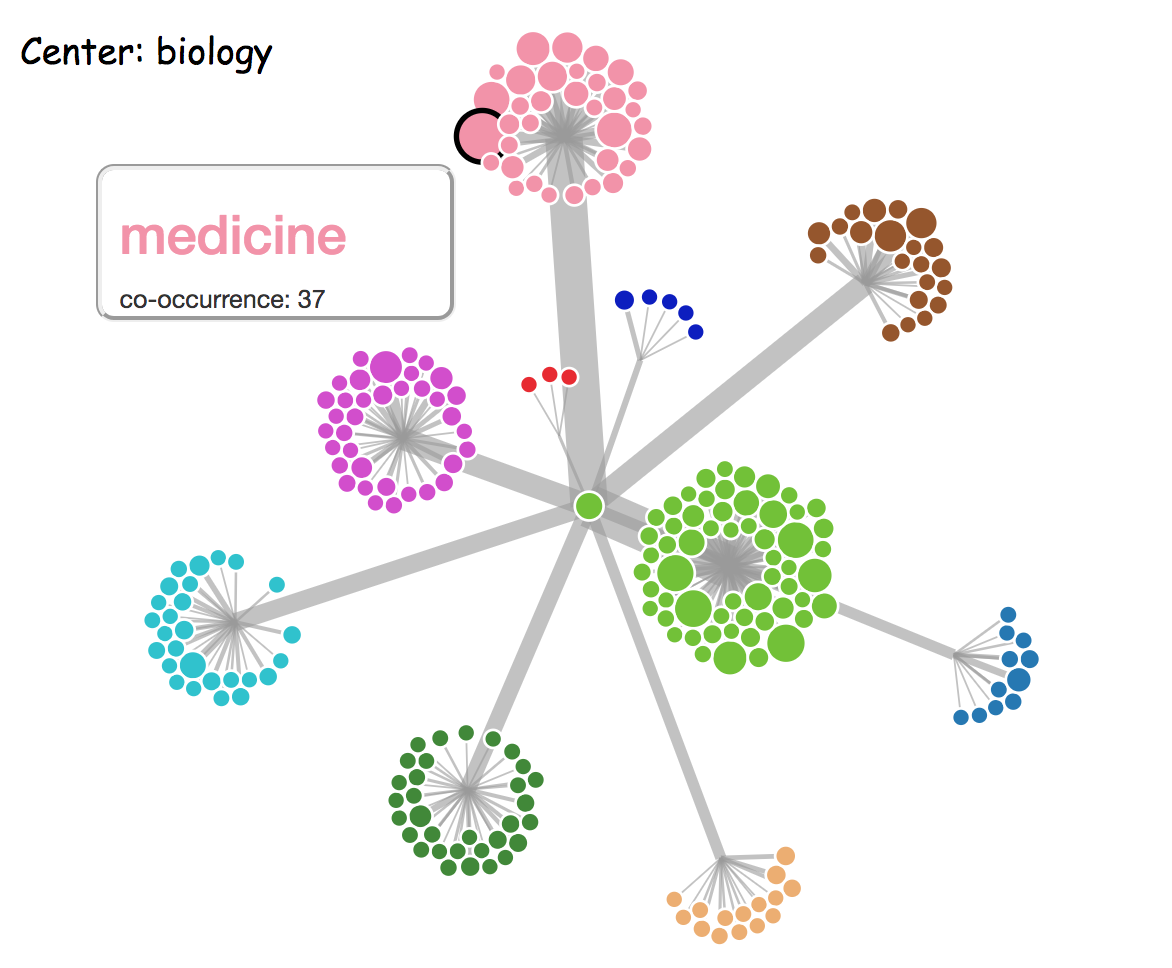
\includegraphics[scale=0.5]{zoomintooltip}
\caption{Tooltip design when we zoom in with center - biology}
\label{fig:tt2}
\end{center}
\end{figure}

\begin{figure}
\begin{center}
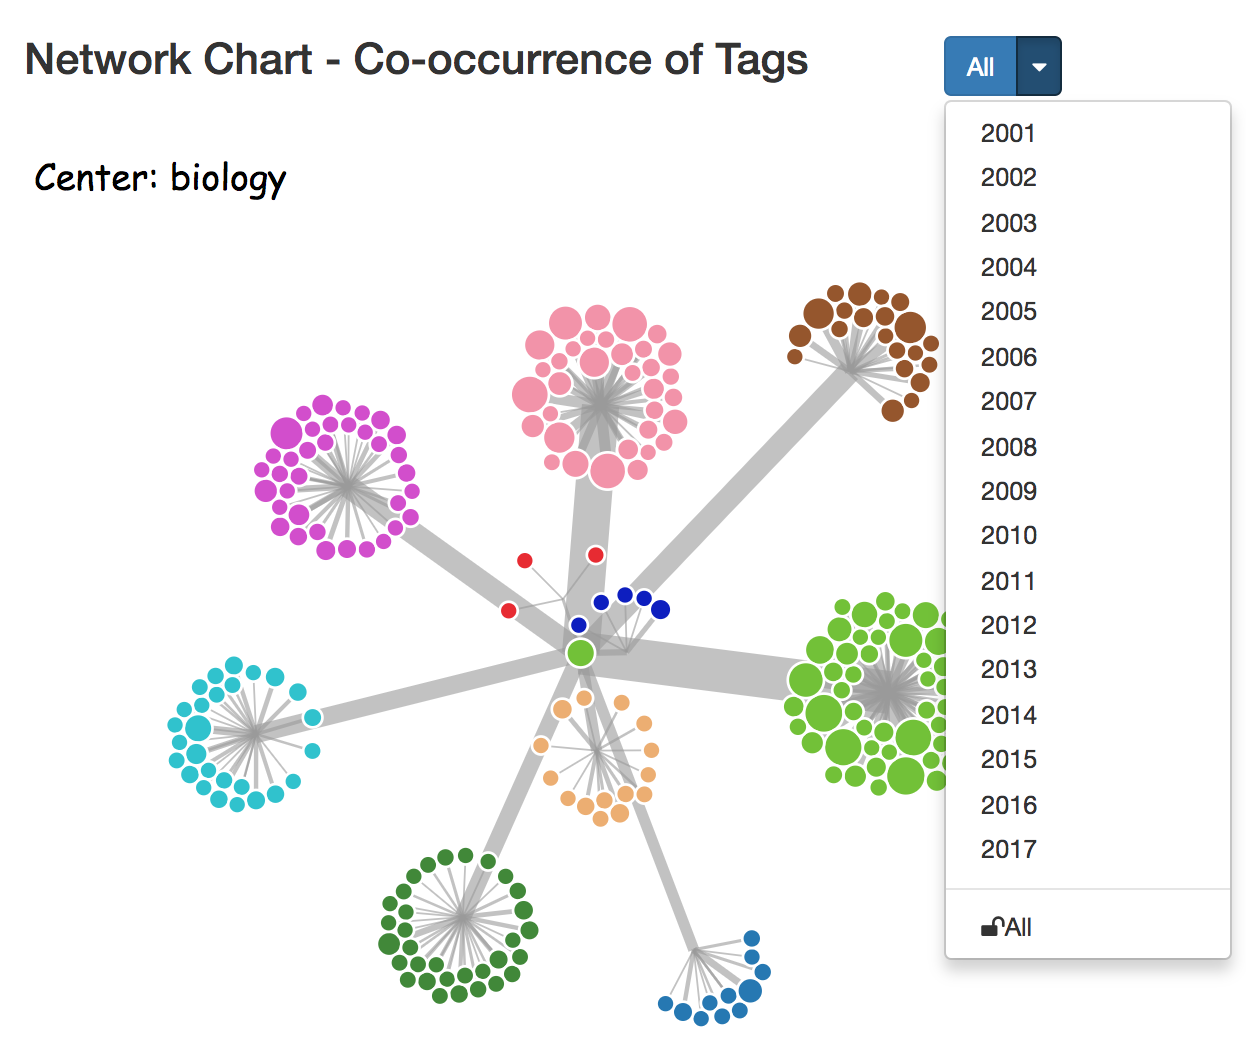
\includegraphics[scale=0.5]{yeardropdown}
\caption{Dropdown list design for choosing year}
\label{fig:yeardropdown}
\end{center}
\end{figure}

\begin{figure}
\begin{center}
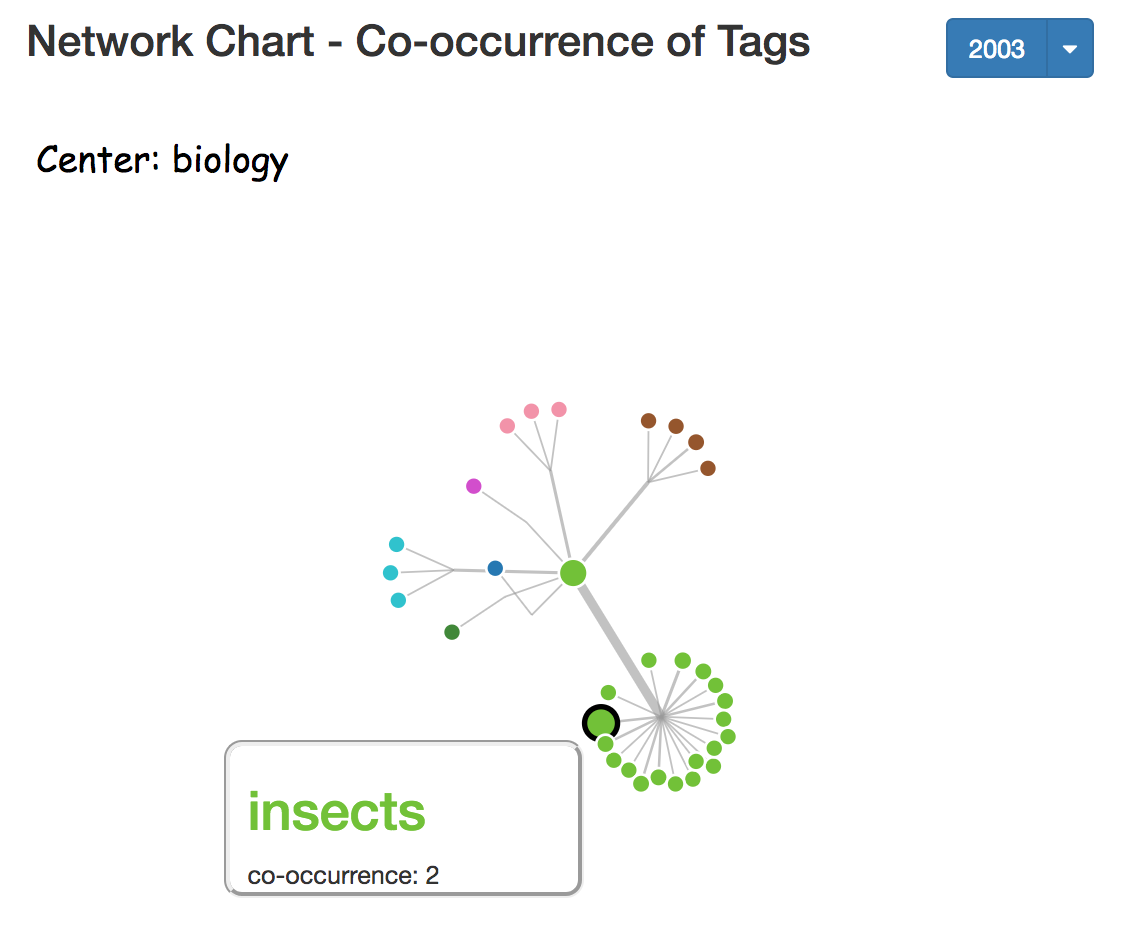
\includegraphics[scale=0.33]{biology2003}
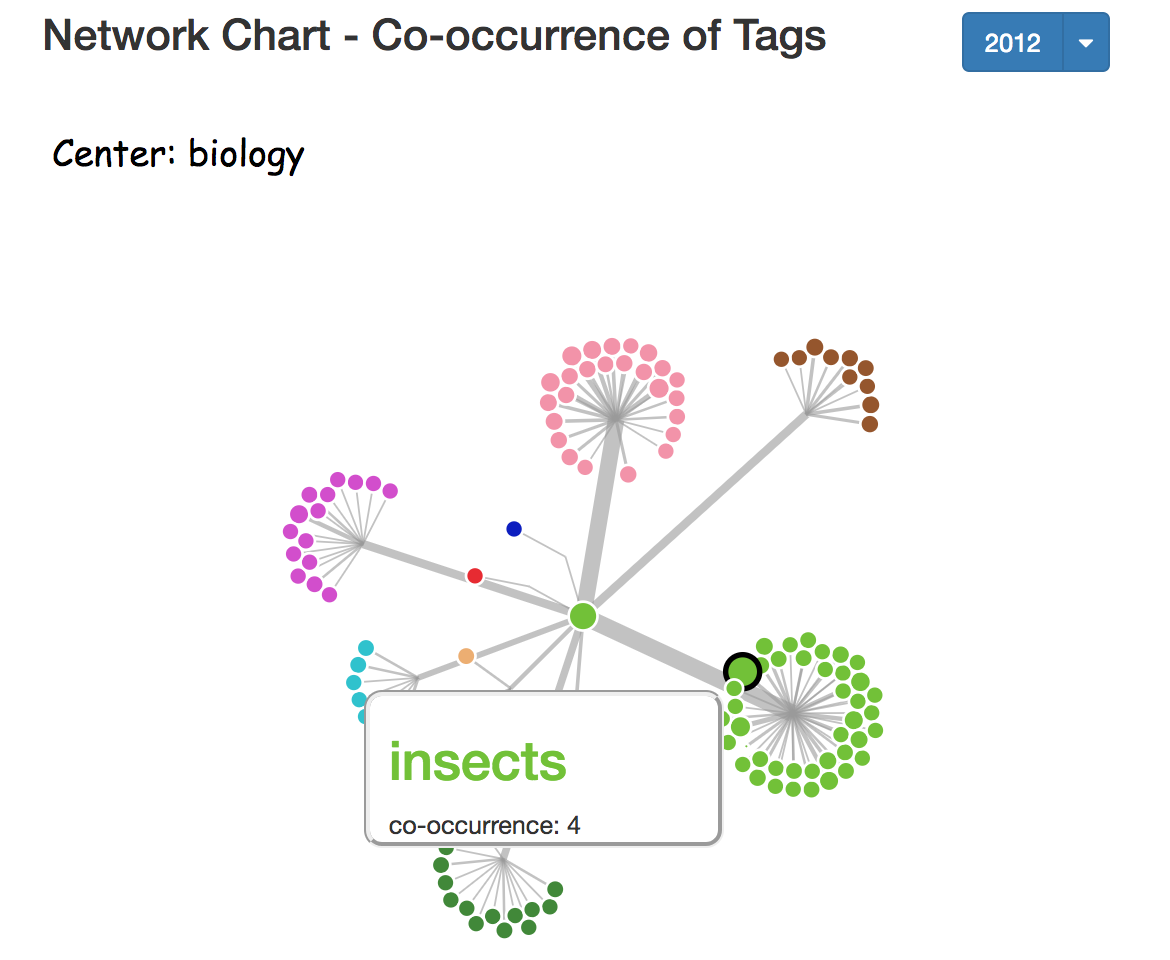
\includegraphics[scale=0.33]{biology2012}
\caption{Comparation of flower chart in 2003 and 2012}
\label{fig:compareyear}
\end{center}
\end{figure}

\subsection{Word Cloud Chart}
\quad After we draw the network chart and color each node according to category, we suddenly find that we did not explain the category and which tags are classified to. Therefore, we decide to add a word cloud chart on the top of page, which provides the information about the members each category includes, and the color of text follow the ordinal color scale we define in network chart. 

\quad In the beginning, the word cloud use a list of buttons for user to select the category, as Figure~\ref{fig:wcbutton1}

\begin{figure}
\begin{center}
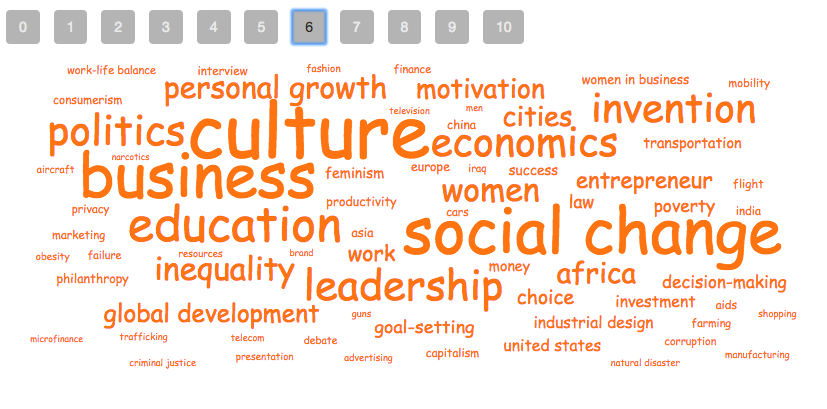
\includegraphics[scale=0.5]{wcbutton1}
\caption{Word Cloud button design, version 1}
\label{fig:wcbutton1}
\end{center}
\end{figure}

\begin{figure}
\begin{center}
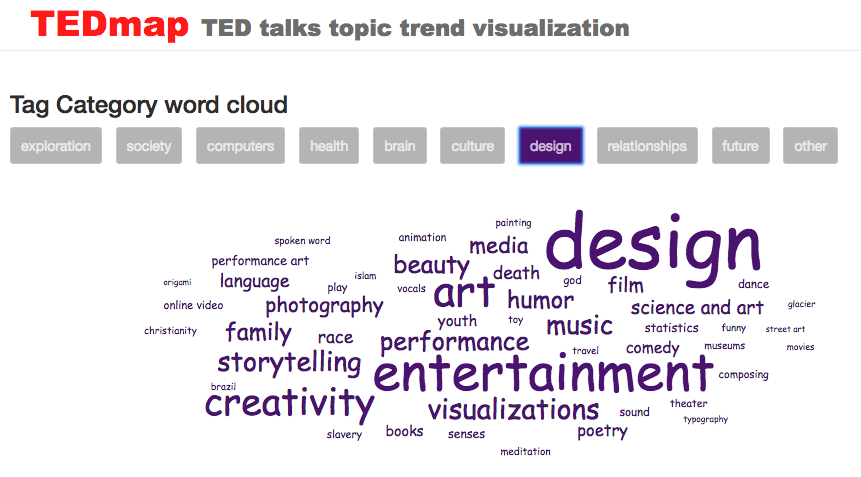
\includegraphics[scale=0.5]{wcbutton2}
\caption{Word Cloud button design, version 2}
\label{fig:wcbutton2}
\end{center}
\end{figure}

\begin{figure}
\begin{center}
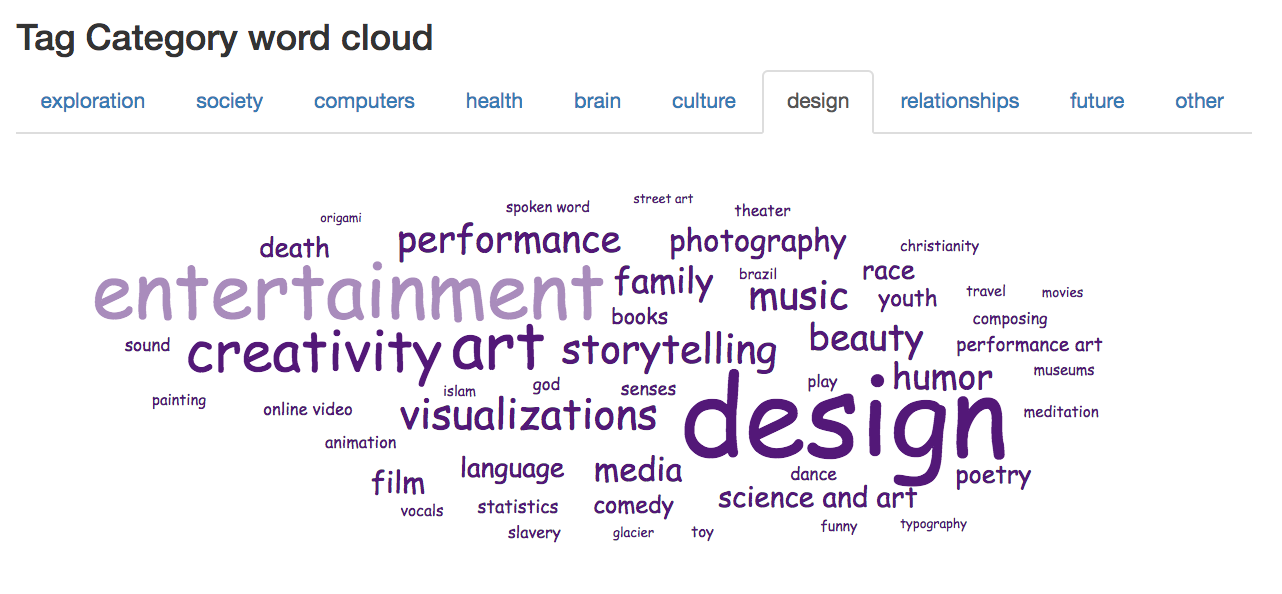
\includegraphics[scale=0.5]{wcbutton3}
\caption{Word Cloud button design, version 3}
\label{fig:wcbutton3}
\end{center}
\end{figure}

\subsection{Line Chart}
\quad  We need to present the video numbers of tags from 2002 to 2017 on our Line Chart design. We originally choose to use color as our channel to discern data, but soon we realize that colors are not enough for our hundreds of tags even if we use a gray scale on each hue. Therefore, we decide to add symbols\cite{d3.symbol} in the d3.js. on our Line Chart. Since symbols and the line on the Line Chart are both made by path element, it is more convenient for our implementation. The final design is show in Figure \ref{fig:linechart}


\begin{figure}
\begin{center}
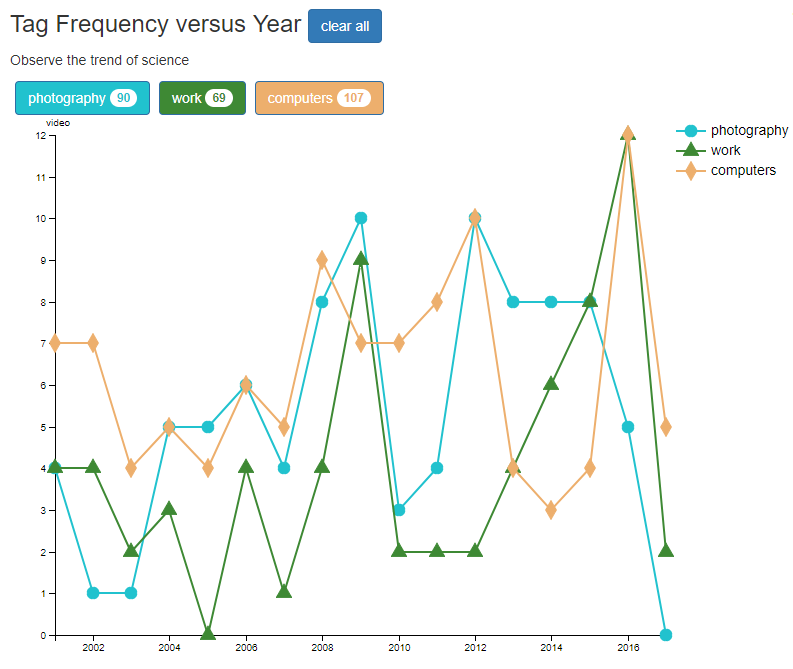
\includegraphics[scale=0.4]{linechart}
\caption{Line Chart.}
\label{fig:linechart}
\end{center}
\end{figure}



\subsection{Button of Line Chart}
\quad To better manage the interaction between these chart, we present Buttons Object. When users click on the Network or the Text Cloud, the clicked tag will be append into the set object behind the button. Once users click the button, we remove the tag in the set object. We easily and elegantly solve the problem of letting users have to many interface to interact with our components. We show our design flow in Figure \ref{fig:topo}


\begin{figure}
\begin{center}
\includegraphics[scale=0.1]{"topo".jpg}

\caption{Flow Chart of our design.}
\label{fig:topo}
\end{center}
\end{figure}


\quad To increase connection of the Line Chart and the Table, we also need to let the Buttons have some hover event that can connected the Line Chart and the rows in the Table.

\subsection{Video List Table}

\quad The requirement in the Table is to show the rest information that we haven't  show  in those components above. Table is the best way for our case. 

We originally try to draw a svg table for the transition purpose. However, it need to much design and it is too hard to put all the information on the drawed svg table. Figure \ref{fig:oldtable} and Figure \ref{fig:newtable} is our different two versions of design in Video List Table.

\begin{figure}
\begin{center}
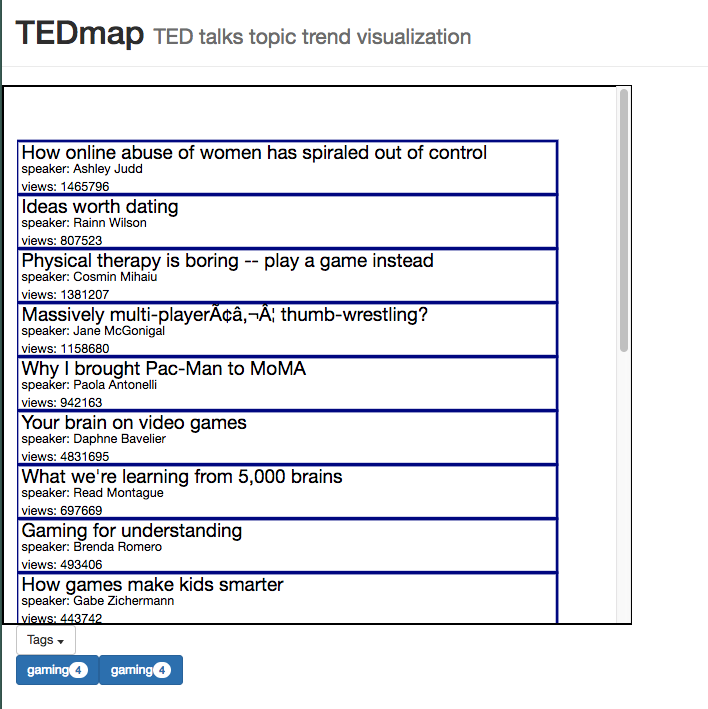
\includegraphics[scale=0.2]{table}
\caption{Our original Table Design.}
\label{fig:oldtable}
\end{center}
\end{figure} 

\begin{figure}
\begin{center}
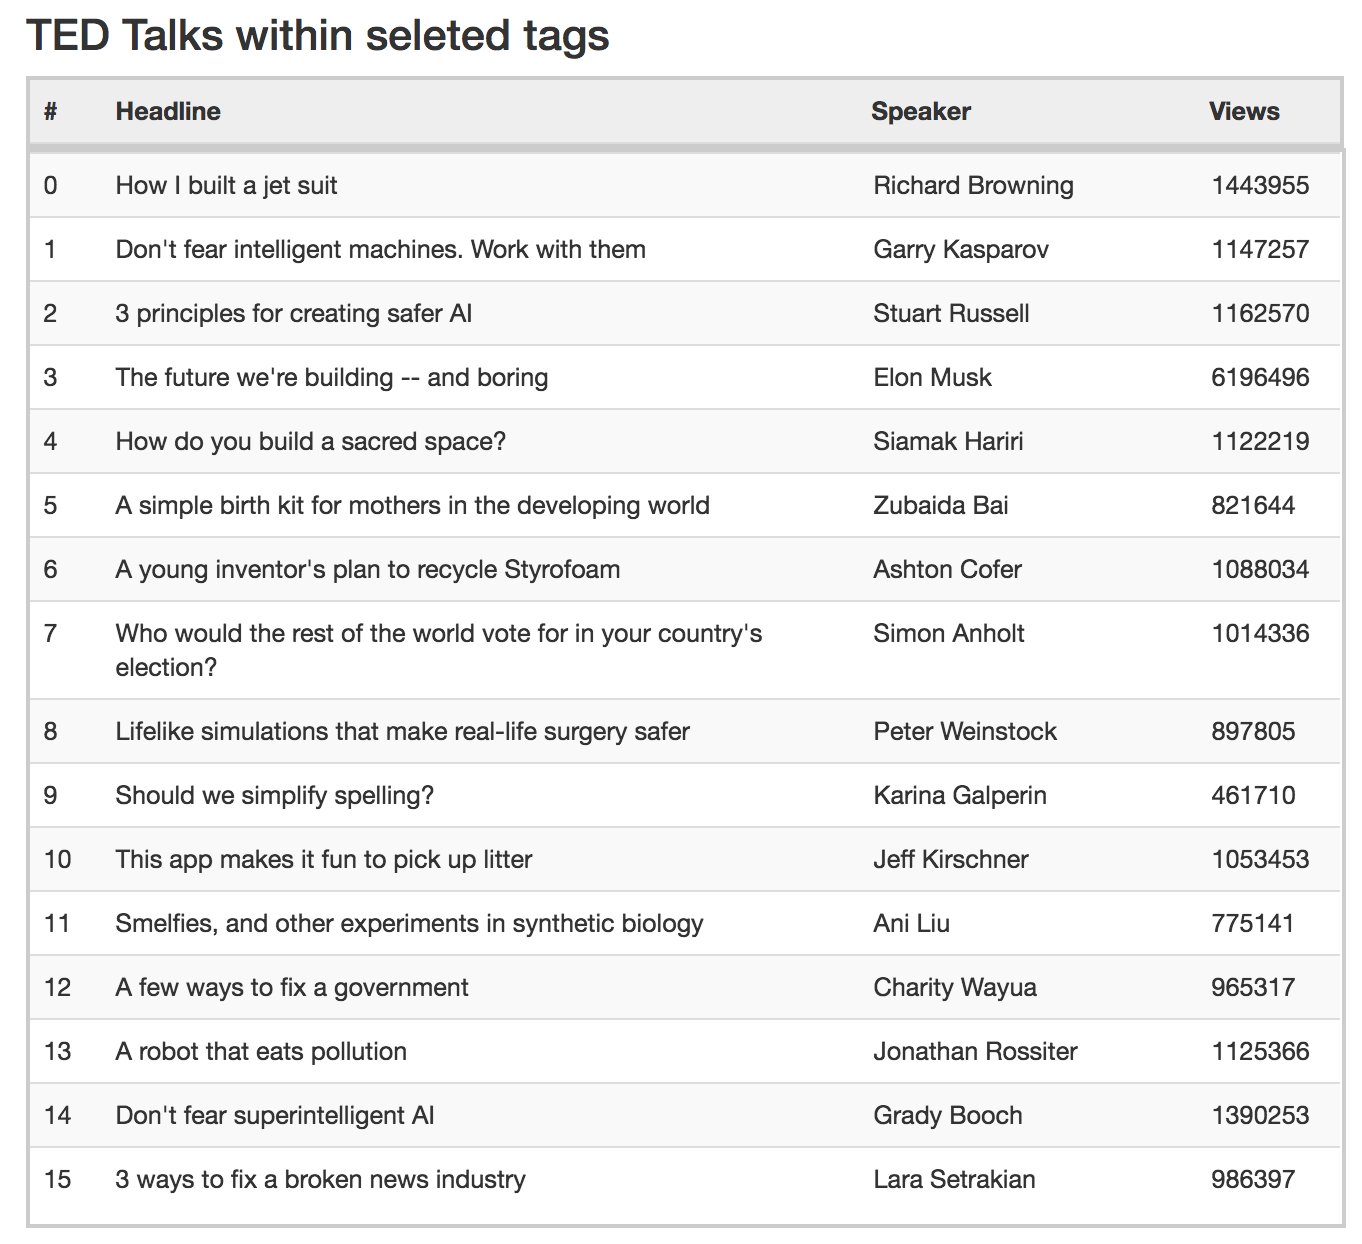
\includegraphics[scale=0.2]{newtable}
\caption{Our new Table Design.}
\label{fig:newtable}
\end{center}
\end{figure} 

\subsection{Radar Chart}
\quad After finish our must-have components, we decide to add an interesting Radar Chart on the tooltips of the Table. Comparing to the line chart on the official of TED(Figure \ref{fig:rateonted}), we believe that our Radar Chart is more likely to catch users eyes and let user understand the meaning of the rates of those videos.

\begin{figure}
\begin{center}
\includegraphics[scale=0.4]{"rateonted1".png}
\caption{The Rate chart show on TED official website.}
\label{fig:rateonted}
\end{center}
\end{figure} 

\begin{figure}
\begin{center}
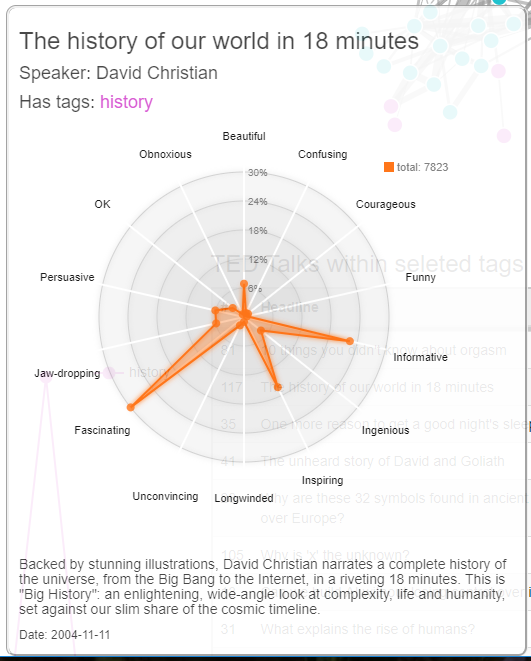
\includegraphics[scale=0.3]{radar}
\caption{Radar Chart.}
\label{fig:radar}
\end{center}
\end{figure} 

%\appendix

\chapter{Implementation}
\section{Overview}
\quad Figure \ref{fig:topo} show the topology of our visualization web page. User can run through Word Cloud, Network Chart, Line Chart, Video List Table to either finding their next interested video, or understanding the trends of popular topic in TED in the recent decade. All of the components are interactive and the usage are easy to come up with.

When users connects to our website, they will intuitively see the Word Cloud and The Network Chart. In the Word Cloud, the texts are scattered and sized by their popularity. The bigger text, the more popular topics in TED video. When users cursor go over the text, tooltips will show on the Network Chat. Also, the cursor will turn to a pointer, mean the user can click. After clicking either on the Word Cloud or the Network Chart, the component below will react dependently on the tags they click so the user will see the change and lead to the next two component we have. Besides, the users can double click on the Word Cloud or the Network Chart to turn the Network Chart into Flower Chart. Flower Chart allow users to connect their interested tag with other tags it may have. This help users to find their next tags they may want to add on the Buttons. The number next to the a button is the number of video that has this tag.

Our Line Chart and Video List Table come to their eyes when the user scroll down in the page. As we mention above, all of the components in our design are able to interact intuitively. So the users' next step would be try to hover the things we have here. In the Line Chart, every components is able to interact by the hover events we built and both the Line Chart and Video List Table will react accordingly. This let the user to discover the video in TED website from the topic they are interested in. When the user try to see into the detail on the Video List Table, they can discover the Radar Chart first with the sufficient information along with it. The radar chart can let the users have a first picture of how other people thinks about this video then the user can decide whether to view this video themselves.

\section{Interaction}
\subsection{Network Chart}
\subsection{Word Cloud}
\subsection{Line Chart}

\quad The Line Chart shows the number of videos for selected tags year from 2002 to 2017. The X axis is the number, the y axis is the year, and the symbol show the exact position of which year has how many video published. In this Line Chart, we mainly use d3 axis and d3 path to render the chart. The lines and the symbols in the chart is path attribute, and the text is text attribute. We also implement mouseover event to increase interaction between the Line Chart and the Video List Table. Once the cursor over the path attribute, the stroke width of line and the symbol will increase so users can feel the difference.

Figure \ref{fig:linechart} On the right-top we implement a small icon to indicate the relationship between the tag name and the symbol-colored line.

\subsection{Buttons}

\quad We have to deliver a progress in a short period of time. So in our cooperation, it is better to have some interfaces like the Buttons to assist us to manage and test our result we had built. Behind the Buttons is a Javascript Set, so no identical button will be selected repeatly. We need to be able to increase and remove buttons in our web page. We came up on using click event to achieve the remove function.

\begin{figure}
\begin{center}
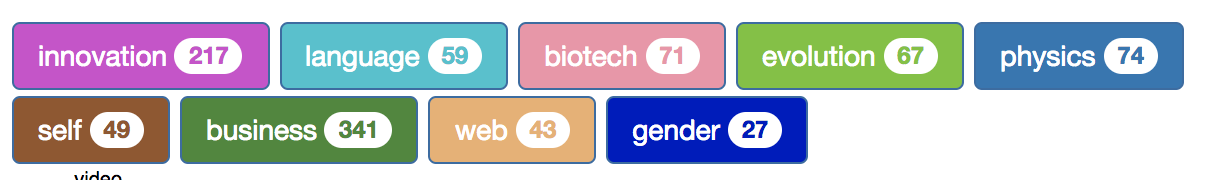
\includegraphics[scale=0.6]{buttons}
\caption{Buttons with a video numbers relating to the tag name.}
\label{fig:buttons}
\end{center}
\end{figure}

Figure \ref{fig:buttons} show our implementation for the Buttons. The little badge with a number behind the tag name shows how many video have the tag in that button.




\subsection{Video List Table}
\quad The information we need to put in the Video List Table is all the other information the user might know for a TED video. Due to the limitation of the space, we agreed on leaving some of the data in the Table and adding d3 tooltip to show further information. This method has many advantage. First, user will have less distraction on the information on the page. Second, instead of dumping all the data to the user, the user can go deeper if they want.

\begin{figure}
\begin{center}
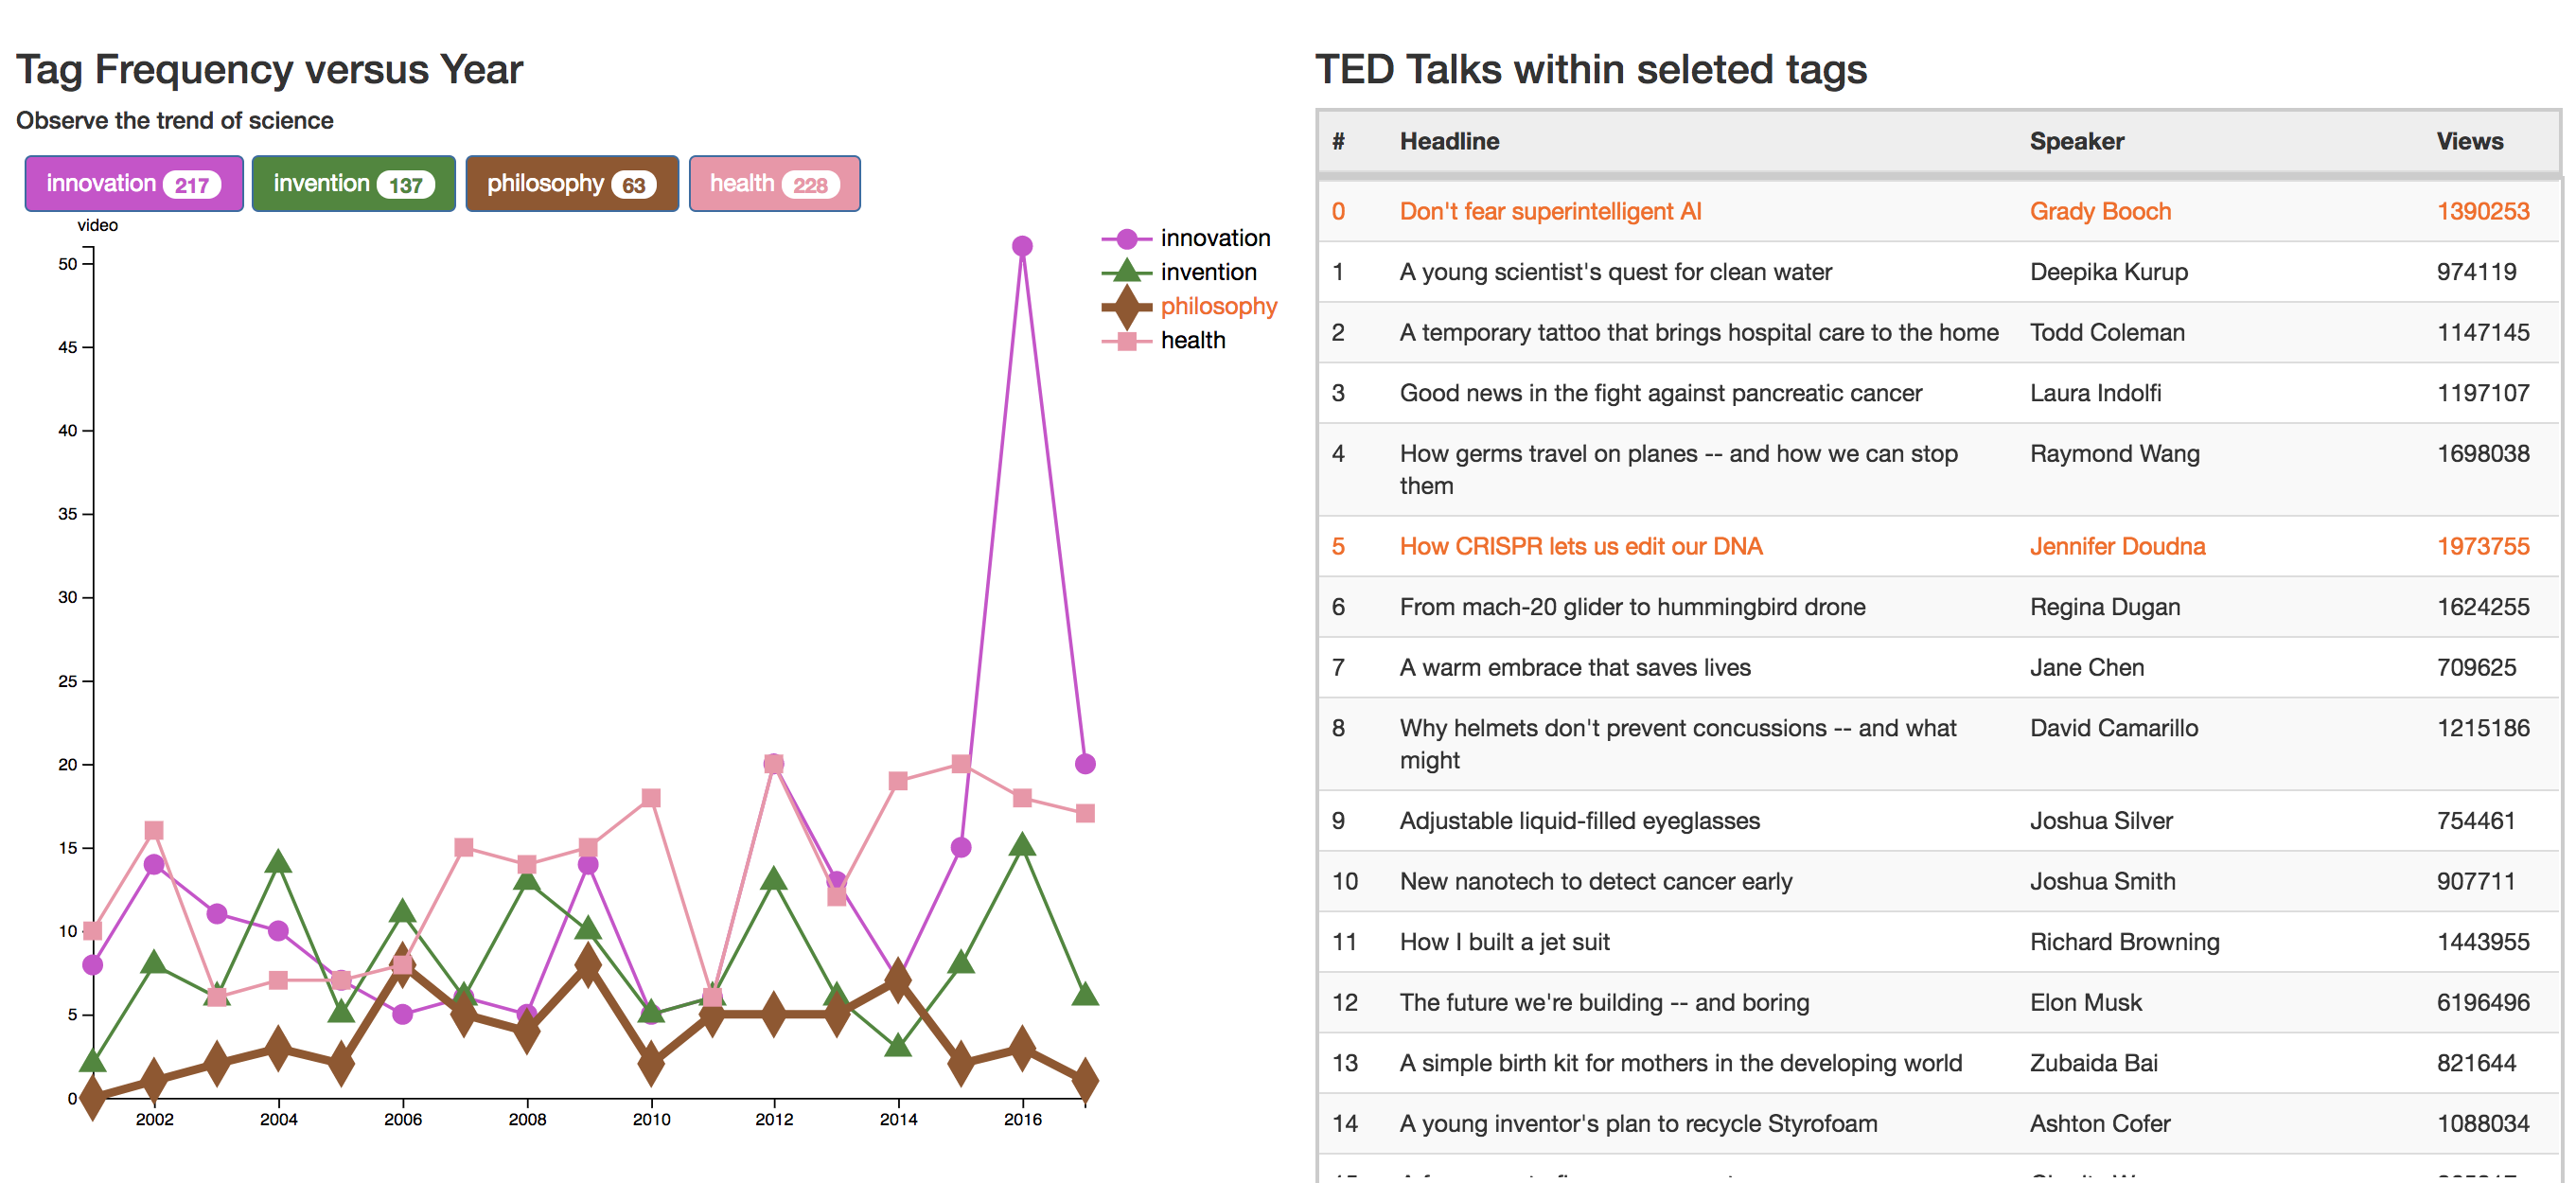
\includegraphics[scale=0.3]{changecolor}
\caption{The hovered tag on the Line Chart will be mark in both the Line Chart and the Video List Table.}
\label{fig:changecolor}
\end{center}
\end{figure} 


To assist user to find their result, we also implemented the sorting feature for the table. The only thing users need to do is click on the header of each column in the table. Figure \ref{sort} show the head of the table that sorted by the speaker name.

\begin{figure}
\begin{center}
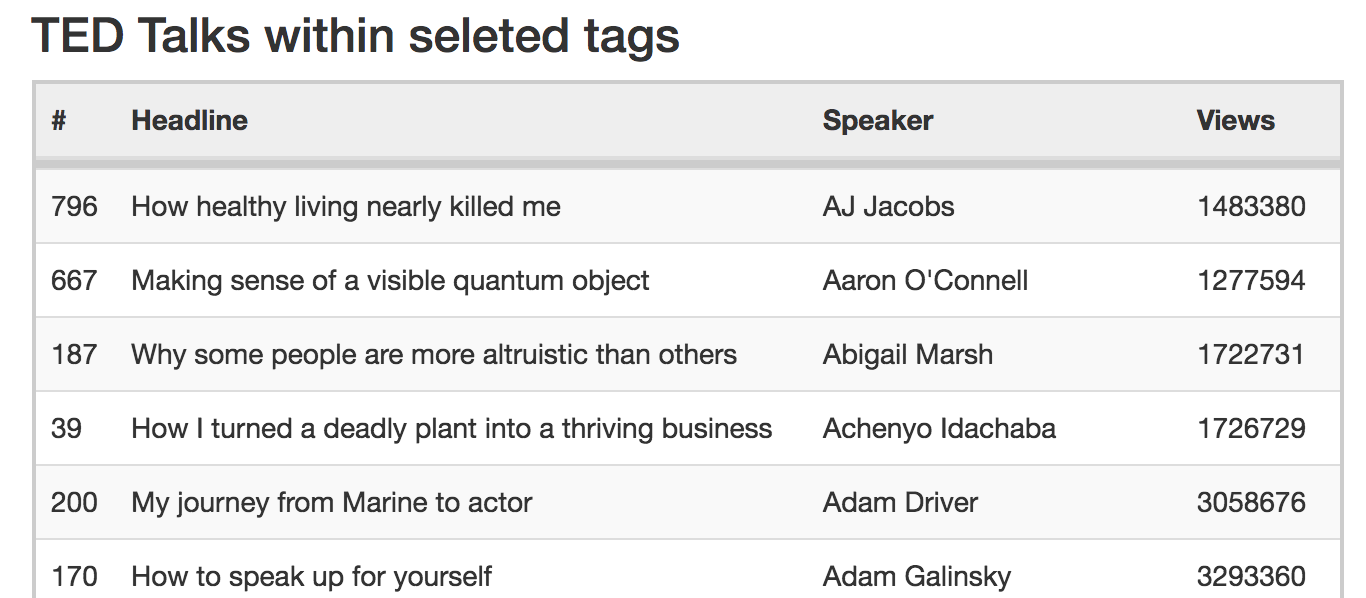
\includegraphics[scale=0.6]{sort}
\caption{Video List Sorted by Speaker Name.}
\label{fig:sort}
\end{center}
\end{figure}

\subsection{Radar Chart}
\quad The Radar Chart is something beyond our optional plan in the proposal: We came up with this idea when implementing the code. The Radar Chart has to show the approximated comments to a video from the massive audience perspectives. The precise number of votes is not important, while the big picture, which is the percentage is crucial if a user just browsing through our website. Therefore, we choose to use radar chart to realize this thought. The scale of our radar chart change dependently on the highest percentage.
 In the Radar Chart, we have fourteen X axis and a Y axis. Each X axis means a adjective according to the official website. The Y axis show the value of each adjective by the distance to the origin of the center.


\section{Flow-Chart}

\chapter{Evaluation}
\section{Solution in our question}
 
\bibliographystyle{acm}
%%\bibliography{nfv.bib}
\bibliography{biblio.bib}

\end{document}
